\documentclass{../cs-classes/cs-classes}

\title{Extending Layerwise Relevance Propagation using Semiring Annotations}
\author{
    \textbf{Antoine Groudiev}\\L3, DI, ENS
    \and
    \textbf{Silviu Maniu}\\Slide Team, LIG, UGA
}

\addbibresource{report.bib}
\graphicspath{{../cs-classes}{../images}}

\begin{document}
\begin{abstract}
    Recently, neural networks allowed computers to solve numerous problems from diverse machine learning fields, such as natural language processsing and computer vision. Compared to traditional algorithms, machine learning models have proven both more successful and more difficult to interpret. Neural networks are considered as black boxes unable to easily explain themselves, that is justifying the reasons that led them to make a prediction. Layer-wise Relevance Propagation (LRP) is a technique that has been introduced to provide explanability by identifying the input features relevant to the output choice. In parallel, research in the databases field developed annotations techniques to compute provenance for queries. In this paper, we extend LRP propagation rules to semiring-based provenance annotations of the network, for LRP to gain in expressivity.
\end{abstract}

\section{Introduction}
\subsection{Problem statement}
Deep neural networks have proven successful for solving with high accuracy machine learning problems. The expressivity of the class of functions generated by neural networks, combined with the relative simplicity of their training, make such models versatile tools to learn the relationship between the inputs and outputs of a dataset.

However, this versatility comes at the cost of poor interpretability: a neural network simply represents a function from one high-dimensional space to another, but provides no justification nor explanation for a given execution. If metrics such as the accuracy over a testing set provide confidence in the fact that the model is able to correctly classify inputs similar to the training set, no guarantee is given that the model generalizes well. Real-world examples show that networks can overfit the input data, or even take shortcuts instead of learning the intended solution \cite{shortcuts}. For the user to have confidence in its predictions, a neural network should therefore be able to highlight the patterns in the input data that it actually learned.

\subsection{Layer-wise Relevance Propagation}
Layer-wise Relevance Propagation (LRP) \cite{bach-2015} has been introduced as a technique to explain an execution of a neural network. LRP is a procedure propagating the output of the function backward in the network, using diverse rules to compute the \emph{relevance} of a neuron depending on the relevances of the neurons of the upstream layer. LRP introduces the notion of \emph{relevance score} for a neuron, intuitively quantifying the contribution of this neuron to the classification of final classification. A high relevance score indicates that the neuron led to the activation of the considered output; a negative relevance score represents neurons that increased the activation of another output neuron instead of the one considered.

\subsubsection{Setup and notations}
In the following, we consider a deep neural network used for a classification task. We assume that it uses the rectifier activation function\footnote{That is $\ReLU(x)=\max(0, x)$, where ReLU stands for \emph{Rectified Linear Unit}.}, which is the case in most applications. To ease the notation, we will not consider biases but instead assume that the first neuron of each layer represents the bias. 

Let $L$ be the number of layers of the network, including the input and output layers. We denote by $\left(a^{(l)}_k\right)_k$ the activations of the network. Notably, $\left(a^{(1)}_k\right)_k$ is the input data, and $\left(a^{(L)}_k\right)_k$ is the ouput prediction. We denote by $\left(w^{(l)}_{j, k}\right)_{j, k}$ the weights connecting the $l$-th layer to the $(l+1)$-th layer. To simulate the biases using only weight matrices, we set:
\begin{equation*}
    \forall l\in\iset{1}{L}, \quad a^{(l)}_0 = 1
\end{equation*}
and we define $w^{(l)}_{0, k}$ to be the bias of the $k$-th neuron of the $(l+1)$-th layer. The forward propagation rule of a deep rectifier network is therefore:
\begin{equation}
    \forall l\in\iset{1}{L-1}, \forall k, \quad a^{(l+1)}_k = \ReLU\left(\sum_{j=0}a^{(l)}_j w^{(l)}_{j, k}\right) = \max\left(0, \sum_{j=0}a^{(l)}_j w^{(l)}_{j, k}\right)
\end{equation}

We denote by $R^{(l)}_j$ the relevance of the $j$-th neuron of the $l$-th layer. We assume that the output layer represents a one-hot encoding, that is that the belonging of the input to the $i$-th class is represented by an output vector is of the form $(0, \dots, a^{(L)}_i, \dots, 0)$, where the only non-null coefficient is in the $i$-th position. Finally, we denote by $y$ the label of a classified input. To the label $y=i$ is associated the output vector $(0, \dots, a^{(L)}_i, \dots, 0)$.

\subsubsection{Propagation rules}
Relevance scores are initialized for the output layer, and are set to the output activation for the correct class, that is:
\begin{equation}
    R^{(L)}_i = \begin{cases*}
        a^{(L)}_i & if $i = y$\\
        0 & otherwise
    \end{cases*}
\end{equation}

The simplest LRP rule is called LRP-0. It propagates the relevance to a neuron of the lower layer proportionnaly to its contribution to each of the neuron of the next layer:
\begin{equation}
    R^{(l)}_j = \sum_{k}\frac{a^{(l)}_jw^{(l)}_{j, k}}{\sum_{j'}a^{(l)}_{j'}w^{(l)}_{j', k}} R^{(l+1)}_k
\end{equation}
The denominator $\sum_{j'}a^{(l)}_{j'}w^{(l)}_{j', k}$ guarantees a conservation property, that is that for any layer $l$:
\begin{equation*}
    \sum_j R^{(l)}_j = \sum_k R^{(l+1)}_k
\end{equation*}
This allows to keep the information regarding the total activation of the final layer.

The application of this simple rule can lead into noisy results that do not scale well. An overview of variations of LRP-0 is provided by \cite{montavon-lrp}; not all rules are suitable for all layers. Complex deep neural networks architectures benefit from enhanced rules such as LRP-$\epsilon$ or LRP-$\gamma$, which provide more stable explanations.

Notably, the input layer must be handled using a different rule, since it does not receive its input from ReLU activations, but directly from the input data. The $z^\mathcal{B}$ rule is used in \cite{montavon-lrp} to propagate from layer 2 to 1 (input layer):
\begin{equation}
    R^{(1)}_j = \sum_{k} \frac{x_kw_{j, k} - l_jw^+_{j, k} - h_jw_{j, k}^-}{\sum_{j'}x_kw_{j', k} - l_jw^+_{j', k} - h_jw_{j', k}^-} R^{(2)}_k
\end{equation}
where $(\cdot)^+=\max(0, \cdot)$, $(\cdot)^-=\min(0, \cdot)$. The parameters $l_i$ and $h_i$ respectively define the theoretical minimum and maximum values of the inputs $x_i$. For instance, we might have $l_i=0$ and $h_i=255$ for pixels over 8 bits.

\subsubsection{LRP results and pertinence}
Previous works (\cite{bach-2015}, \cite{montavon-lrp}), as well as the methods that we will introduce later on, were experimentaly tested on models trained over two datasets: fully-connected networks trained on the MNIST handwritten digits dataset \cite{mnist-dataset}, and deep convolutional networks pre-trained on the ImageNet visual database such as VGG-16 \cite{vgg}.

\autoref{fig:mnist-lrp} shows relevance for a simple model: a fully-connected deep rectifier network with layers of sizes $28\times28$, $300$, $100$ and $10$, trained on the MNIST dataset. Pixels highlighted in red have a positive relevance while blue pixels have a negative relevance. As expected, the relevant pixels to classify this image as a \texttt{0} are the white pixels in the input image.

\begin{figure}[H]
    \centering
    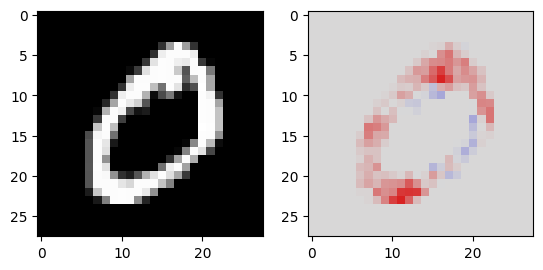
\includegraphics[width=.5\textwidth]{mnist-lrp.png}
    \caption{Input image and pixel-wise explanation of the output neuron \texttt{0}}
    \label{fig:mnist-lrp}
\end{figure}

\autoref{fig:castle-lrp} provides a visualization for a more complex example, an execution of the VGG-16 network over a $224\times224$ image. 
\begin{figure}[H]
    \centering
    \begin{minipage}[c]{.49\textwidth}
        \centering
        
\includegraphics[width=.65\textwidth]{castle.jpg}
    \end{minipage}
    \hspace*{-2.5cm}
    \begin{minipage}[c]{.49\textwidth}
        \centering
        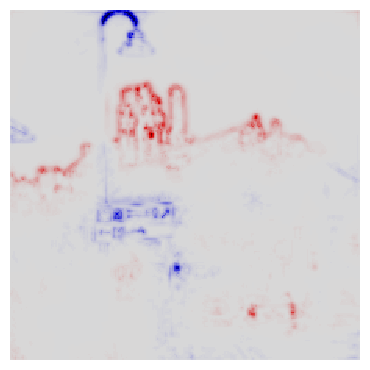
\includegraphics[width=.65\textwidth]{castle-lrp.png}
    \end{minipage}
    \caption{Input image and relevance for the class "\texttt{castle}" of the VGG-16 network}
    \label{fig:castle-lrp}
\end{figure}
Note that the castle part of the image is highlighted in red as intended. Furthermore, both the street sign and the street light have strong negative relevance; those two objects correspond to other classes of the ImageNet dataset (\texttt{street sign (919)} and \texttt{traffic light (920)}). Those two elements of the image would have positive relevance for LRP starting from the output neurons \texttt{919} and \texttt{920}.

% TODO: double MNIST?

\subsection{Semiring-based provenance annotations}
In parallel, the notion of data provenance in databases theory developed formal solutions to a similar problem to ours. Data provenance aims at \emph{explaning} a query by highlighting the tuples in the original database that led to the presence of a certain tuple in the query result. If contexts are different, deep neural networks explanation and data provenance share the same general setup: identifying a subset of the input that directly implied a certain output.

A framework to approach data provenance is \emph{provenance semirings}, introduced in \cite{green-2007}, annotates tuples using abstract elements of a semiring and apply semiring operations to the tuples appearing in the query. As the query is executed, information about the provenance of the intermediate results is aggregated, resulting in an abstract formula that can be concretized by substituting abstract elements and operations by a concrete semiring. Similarly, in the context of graph databases, edges can be annotated to derive a variety of properties of the query result. \cite{ramusat-prov}

In the following, we provide a mathematical definition of a semiring as well as semiring examples suited for the application to deep neural networks.

\begin{definition}[Semiring]
    A \emph{semiring} is an algebraic structure generalizing the notion of rings. A semiring $(\mathbb{K}, \oplus, \otimes, \mathbf{0}, \mathbf{1})$ is composed of a set $\mathbb{K}$, binary operators $\oplus$ and $\otimes$ such that $\otimes$ distributes over $\oplus$, verifying the following properties:
    \begin{itemize}
        \item $(\mathbb{K}, \oplus, \mathbf{0})$ is a commutative monoid
        \item $(\mathbb{K}, \otimes, \mathbf{1})$ is a monoid such that $\mathbf{0}$ is absorbing
    \end{itemize}
\end{definition}

\begin{example}
    $(\R, +, \times, 0, 1)$ is a semiring. While it has no direct interpretation is the context of databases, we will see that is corresponds to the basic real-valued LRP.
\end{example}

\begin{example}[Boolean semiring]
    $(\{\bot, \top\}, \lor, \land, \bot, \top)$ is a semiring. Its use in databases provenance interprets as the existence of a path between two vertices, using edge weights as the number of different paths between two adjacent vertices. 
\end{example}

\begin{example}[Counting semiring]
    $(\mathbb{N}, +, \times, 0, 1)$ is a semiring. For a non-cyclic graph database, its use allows to compute the total number of paths between two vertices, using edge weights as the number of different paths between two adjacent vertices.
\end{example}

\begin{example}[Viertbi semiring]
    $([0, 1], \max, \times, 0, 1)$ is a semiring. For a non-cyclic graph database where the annotations are interpreted as a \say{confidence} measure, its use allows to compute the confidence score of the result of a query.
\end{example}

\section{Extending LRP using Semiring Annotations}
\subsection{Semiring generalization of the LRP rule}
\subsection{Results over the MNIST dataset}
\subsubsection{Boolean Semiring}
\subsubsection{Counting Semiring}
\subsubsection{Viterbi Semiring}

\section{Handling of convolutional neural networks}
\subsection{Computing relevance for convolutional layers}
\subsubsection{Forward pass}
\subsubsection{Gradient expression of LRP}
\subsubsection{Implementing LRP without automatic differentiation}

\subsection{Results for the VGG-16 network}

\subsection{Thresholds choice}

\section{Applications}
\subsection{Image mask computation}
\subsection{Network pruning using LRP ranking}
\subsection{Comparison to image perturbation}

\newpage
\nocite{*}
\printbibliography

\end{document}